%!TEX root = ./slopecd.tex

\section{Theory}\label{sec:theory}
%%%%%%%%%%%%%%%%%%%%%%%%%%%%%%%%%%%%
\subsection{Coordinate Descent for SLOPE}%
\label{sec:coordinate-updates}

\mathurin{Suggestion: \\
Proximal coordinate descent cannot be applied to \Cref{pb:slope} because it is not separable.
However, if the clusters $\mathcal{C}_1, \ldots, \mathcal{C}_m$ of the solution $\hat \beta$ were known together with its sign, then the values $c_1, \ldots, c_m$ taken by $\hat \beta$ on the clusters could be equivalently computed by solving :
\begin{problem}
\min_{x \in \bbR^m}
F \left(\sum_{i=1}^m \tilde{X}_i x_i \right)
+ \sum_{i=1}^m (\sum_{\lambda \in \lambda^{\mathcal{C}_i}} \lambda) x_i \enspace,
\end{problem}
where $\tilde{X}_{\mathcal{C}_i} = \sum_{j \in \mathcal{C}_i} X_j \sign (\hat \beta_j)$.
Hence, the idea of our algorithm is to intertwine steps that identify the clusters, and large coordinatewise steps on these clusters.
}
Based on this observation, we derive a coordinate descent algorithm for minimizing the SLOPE problem~\eqref{pb:slope} with respect to the coefficients of a single cluster at a time.
First observe that we can write \Cref{pb:slope} as \mathurin{To discuss:  we restrict to quadratic datafit? in the intro there's a generic df and our strategy would be adapted to it, it's just block coordinate descent with varying blocks}
\[
  \begin{aligned}
    P(\beta)
     & =  \frac{1}{2} \lVert y - X\beta\rVert_2^2 + J(\beta)                        \\
     & = \frac{1}{2} \lVert y - X_{\bar{\mathcal{C}_k}} \beta_{\bar{\mathcal{C}_k}}
    - \big(X_{\mathcal{C}_k} s_{\mathcal{C}_k}\big)c_k  \rVert_2^2
    + |c_k|\sum_{j \in {\mathcal{C}_k}} \lambda_{(j)^-}
    + \sum_{j \notin {\mathcal{C}_k}} |\beta_j|\lambda_{(j)^-}                      \\
     & = \frac{1}{2} \lVert \tilde r - \tilde x c_k \rVert_2^2
    + |c_k|\sum_{j \in {\mathcal{C}_k}} \lambda_{(j)^-}
    + \sum_{j \notin {\mathcal{C}_k}} |\beta_j|\lambda_{(j)^-}                      \\
  \end{aligned}
\]
with \( \tilde x_k = X_{\mathcal{C}_k} s_{\mathcal{C}_k}\) and
\(\tilde r_k = y - \tilde y_k = y - X_{\bar{\mathcal{C}}_k} \beta_{\bar{\mathcal{C}}_k} \in \bbR^n\).
\mm{do we need $\tilde y _k$ ?}
\mathurin{What is tricky here is that $\beta$ varies so the $C_k$ and $c_k$ vary too. THe notation $C_k(\beta)$ would be too heavy (most of all because $m$ also depends on $\beta$, but so I would avoid writing such computations that are confusing IMO - at least they confused me to be honest)}

\mathurin{I would just say we perform block coordinate descent update/directional updates in the direction of $(\sign \beta)_{\mathcal{C_i}}$
}
We propose a coordinate-wise update that minimizes \(P(\beta)\) with respect to the
clusters' corresponding coefficients one at a time, keeping the relative signs
of the coordinates within each cluster fixed but allowing all of the signs to
flip (simultaneously).

Letting \(\beta\) correspond to a fixed vector, note that
\(\beta_i = s_i c_{(j)^-}\), \(i \in \mathcal{C}_j\) for all
\(i\). Now let \(\tilde{\mathcal{C}}_i\)
correspond to the indices of the \(i\)th cluster for \(\beta\), that is,
\(|\beta_j| = c_i\) for all \(j \in \tilde{\mathcal{C}}_i\).
Next, we let
\begin{equation}
  \label{eq:coordinate-update-beta}
  \beta_i(z) =
  \begin{cases}
    s_k z   & \text{if } i \in \mathcal{C}_k, \\
    \beta_i & \text{otherwise.}
  \end{cases}
\end{equation}
\mathurin{maybe we can write $\beta + z \sign(\beta)_{\mathcal{C}_i}$, where $\sign$ is the sign vector, and restricting indices keeps the dimension (and puts 0 as value of excluded indices).}
This means that \(\beta(x)\) corresponds to a version of \(\beta\) with a
coordinate update for the \(k\)th cluster.

This corresponds to solving the following
one-dimensional problem:

\begin{equation}
  \label{eq:cluster-problem}
  \operatorname*{minimize}_{z \in \mathbb{R}} \left(P_k(z) = \frac{1}{2} \lVert \tilde r - \tilde x z \rVert_2^2 + J_k(z)\right)
\end{equation}
where
\[
  J_k(z) = |z| \sum_{j \in \mathcal{C}_k} \lambda_{(j)^-_z}
  + \sum_{j \notin \mathcal{C}_k} |\beta_j| \lambda_{(j)^-_z}
\]
is the \emph{partial sorted \(\ell_1\) norm} with respect to the \(k\)th cluster and
\mm{new notation; we could write $(j; \beta(z))$ or $(j; \beta + z d)$, $d$ being the direction}
where we write \(\lambda_{(j)^-_z}\) to indicate that the permutation operator \((j)^-_z\)
is defined through \(\beta(z)\).

The optimality condition for this problem is
\[
  P_k'(z; \delta) \geq 0,
\]
where \(P'_k(z; \delta)\) is the directional derivative of \(P_k\).
Note that we have
\[
  P_k'(z; \delta) = \delta\big(\tilde x^T \tilde x z - \tilde r^T \tilde x\big) + J'_k(z; \delta)
\]
since \(\lVert \tilde{r} - \tilde{x}z\rVert_2^2\) is differentiable.

\mathurin{One key aspect of such updates that for me deserves to be emphasized: the clusters will almost all remain the same: they can only change order, or two of them merge.}

Throughout the rest of this section section we will derive a minimizer
solution to \eqref{eq:cluster-problem}. To do so, we will introduce the
directional derivative for the sorted \(\ell_1\) norm with respect to the
coefficient of the \(k\)th cluster. First, however, let
\(C(z)\) be a function that returns the cluster corresponding to \(z\), that is
\[
  C(z) = \{j : |\beta(z)_j| = z\}.
\]
Secondly, we introduce \cref{def:limit-permutation}.
\begin{definition} \mm{cosmetic: I'm not sure this is a definition}
  \label{def:limit-permutation}
  Let there be an \(\varepsilon > 0\) such that
  \begin{equation*}
    \big| c_i - c_j\big| > \varepsilon \quad \forall\, i \neq j
  \end{equation*}
  for a strictly decreasing sequence \(c_1, c_2, ..., c_m\).
  \mm{should the inequality be in the other direction?}
\end{definition}

For an \(\varepsilon\) defined as in \cref{def:limit-permutation}, we have for
\(\delta \in \{-1, 1\}\)\mathurin{This can be hard to parse: $C$ implicitely depends on a vector that determiens clsuters. We can emphasize that  In all this section $\beta$ is fixed and we update only in the direction given by the sign of one cluster. Clusters $C_i$ and $c_i$ are fixed.}
\begin{equation}
  \lim_{h \downarrow 0} C(z + h\delta) = C(z + \varepsilon \delta)
  \quad\text{and}\quad
  \lim_{h \downarrow 0} \lambda_{(i)^-_{z + h\delta}}
  = \lambda_{(i)^-_{z + \varepsilon\delta}}.
\end{equation}
In other words, the order permutation corresponding to \(B(z + h\delta)\)
depends only on \(\delta\) in the limit as \(h\) tends to~\(0\). \mm{typo B for $\beta$?}

\begin{remark}
  As consequence of \cref{def:limit-permutation}, the order
  permutations for \(B(z)\) and \(B(z + \varepsilon \delta)\) differ only for a subset of
  the permutation vectors. The permutation for \(B(h\delta)\) corresponds to
  \[
    \begin{cases}
      \tilde{\mathcal{C}}_1, \dots, \tilde{\mathcal{C}}_{k-1}, \tilde{\mathcal{C}}_{k+1}, \dots, \tilde{\mathcal{C}}_m, C(\varepsilon\delta)                                          & \text{if } c_m > 0 \text{ and } \delta \neq 0, \\
      \tilde{\mathcal{C}}_1, \dots, \tilde{\mathcal{C}}_{k-1}, \tilde{\mathcal{C}}_{k+1}, \dots, C(\varepsilon\delta), \tilde{\mathcal{C}}_m                                          & \text{if } c_m = 0 \text{ and } \delta \neq 0, \\
      \tilde{\mathcal{C}}_1, \dots, \tilde{\mathcal{C}}_{k-1}, \tilde{\mathcal{C}}_{k+1}, \dots, \underbrace{\tilde{\mathcal{C}}_k \cup \tilde{\mathcal{C}}_m}_{C(\varepsilon\delta)} & \text{if } c_m = 0 \text{ and } \delta = 0.    \\
    \end{cases}
  \]
  The permutation for \(B(z + \varepsilon \delta)\), \(z \neq 0\) corresponds to
  \[
    \begin{cases}
      \tilde{\mathcal{C}}_1, \dots, \tilde{\mathcal{C}}_{k-1}, \tilde{\mathcal{C}}_{k+1}, \dots, C(c_i + \varepsilon\delta), \tilde{\mathcal{C}}_i, \dots, \tilde{\mathcal{C}}_m                                          & \text{if } \delta = 1,  \\
      \tilde{\mathcal{C}}_1, \dots, \tilde{\mathcal{C}}_{k-1}, \tilde{\mathcal{C}}_{k+1}, \dots, \tilde{\mathcal{C}}_i, C(c_i + \varepsilon\delta), \dots, \tilde{\mathcal{C}}_m                                          & \text{if } \delta = -1, \\
      \tilde{\mathcal{C}}_1, \dots, \tilde{\mathcal{C}}_{k-1}, \tilde{\mathcal{C}}_{k+1}, \dots, \underbrace{\tilde{\mathcal{C}}_i \cup \tilde{\mathcal{C}}_k}_{C(c_i + \varepsilon\delta)}, \dots, \tilde{\mathcal{C}}_m & \text{if } \delta = 0.  \\
    \end{cases}
  \]
\end{remark}

We are now ready to state the directional derivative of \(J_k\).

\begin{theorem}\label{thm:sl1-directional-derivative}
  The directional derivative of \(J_k\) in the direction \(\delta\) is
  \[
    J'_k(z, \delta) =
    \begin{cases}
      \sign(z)\delta\smashoperator{\sum_{j \in C(z + \varepsilon \delta)}}
      \lambda_{(j)^-_{z + \varepsilon\delta}}                      & \text{if } z = c_i > 0, \\
      |\delta|\smashoperator{\sum_{j \in C(\varepsilon \delta)}}
      \lambda_{(j)^-_{\varepsilon\delta}}                          & \text{if } z = 0,       \\
      |\delta| \smashoperator{\sum_{j \in C(z)}} \lambda_{(j)^-_z} & \text{otherwise}
    \end{cases}
  \]
  with \(\varepsilon\) defined as in \cref{def:limit-permutation}.
\end{theorem}
\begin{proof}
  The directional derivative of \(J_k\) in the direction \(\delta\) is defined as
  \begin{align}
    J_k'(z; \delta)
    = & \lim_{h \downarrow 0} \frac{J_k(z + h \delta) - J_k(z)}{h} \nonumber \\
    = &
    \lim_{h \downarrow 0} \frac{1}{h}
    \left(
      |z + h \delta| \smashoperator{\sum_{j \in C(z + h \delta)}} \lambda_{(j)^-_{z + h \delta}}
      + \smashoperator{\sum_{j \notin C(z + h\delta)}} |\beta_j| \lambda_{(j)^-_{z + h \delta}}
      - |z| \smashoperator{\sum_{j \in C(z)}} \lambda_{(j)^-_z}
      - \smashoperator{\sum_{j \notin C(z)}} |\beta_j| \lambda_{(j)^-_z}
    \right) \nonumber                                                        \\
    = & \lim_{h \downarrow 0}
    \frac{1}{h}
    \left(
      |z + h \delta| \smashoperator{\sum_{j \in C(z + \varepsilon\delta)}} \lambda_{(j)^-_{z + \varepsilon\delta}}
      + \smashoperator{\sum_{j \notin C(z + \varepsilon\delta)}} |\beta_j| \lambda_{(j)^-_{z + \varepsilon\delta}}
      - |z| \smashoperator{\sum_{j \in C(z)}} \lambda_{(j)^-_{z}}
      - \smashoperator{\sum_{j \notin C(z)}} |\beta_j| \lambda_{(j)^-_{z}}
    \right).
    \label{eq:directional-derivative-sl1}
  \end{align}

  First, note that \(J_k\) is differentiable for \(z \notin \{0, c_i\}\), \(i
  \neq k\) and that \(C(z + \varepsilon\delta) = C(z)\), giving
  the directional derivative
  \[
    \delta \sign(z) \smashoperator{\sum_{j \in C(z)}} \lambda_{(j)^-_{z}}.
  \]

  Turning to the case of \(z = \pm c_i\), \(i \neq k\) now, note that we have,
  as a result of the definition of
  \(\varepsilon\)~(\cref{def:limit-permutation}), the following identities:
  \begin{align*}
    C(c_i + \varepsilon\delta)          & \subseteq C(c_i),                                                                                                             \\
    \tilde{\mathcal{C}}_i               & = \widebar{C(c_i + \varepsilon \delta)} \cap C(c_i),                                                                          \\
    C(c_i)                              & = \tilde{C}_i \cup \big(C(c_i + \varepsilon\delta) \cap C(c_i)\big) = \tilde{\mathcal{C}}_i \cup C(c_i + \varepsilon \delta), \\
    \widebar{C(z + \varepsilon \delta)} & = \widebar{C(c_i)} \cup \tilde{\mathcal{C}}_i.
  \end{align*}
  Using this, we can rewrite \eqref{eq:directional-derivative-sl1} as
  \begin{equation*}
    \label{eq:directional-derivative-simplified}
    J'_k(z; \delta)
    = \lim_{h \downarrow 0} \frac{1}{h}
    \left(
      \splitfrac{
      |z + h\delta|\smashoperator{\sum_{j \in C(z + \varepsilon\delta)}} \lambda_{(j)^-_{z + \varepsilon\delta}}
      + |c_i|\smashoperator{\sum_{j \in \tilde{C}_i}} \lambda_{(j)^-_{z + \varepsilon\delta}}
      + \smashoperator{\sum_{j \in \widebar{C(z)}}} |\beta_j|\lambda_{(j)^-_{z + \varepsilon\delta}}
      }{%
      - |z| \smashoperator{\sum_{j \in \tilde{\mathcal{C}}_i}} \lambda_{(j)^-_{z}}
      - |c_i| \smashoperator{\sum_{j \in C(z + \varepsilon\delta)}} \lambda_{(j)^-_{z}}
      - \smashoperator{\sum_{j \in \widebar{C(z)}}} |\beta_j| \lambda_{(j)^-_{z}}
      }
    \right).
  \end{equation*}
  Next, observe that \(\lambda_{(j)^-_{z + \varepsilon\delta}} =
  \lambda_{(j)^-_{z}}\) for all \(j \in \widebar{C(z)}\) and consequently
  \[
    \smashoperator{\sum_{j \in \widebar{C(z)}}} |\beta_j|\lambda_{(j)^-_{z + \varepsilon\delta}} =
    \smashoperator{\sum_{j \in \widebar{C(z)}}} |\beta_j|\lambda_{(j)^-_{z}}.
  \]
  Moreover, note that, since \(z = \pm c_i\), there exists a permutation corresponding to
  \(\lambda_{(j)^-_{z}}\) such that
  \[
    |z|\smashoperator{\sum_{j \in \tilde{C}_i}} \lambda_{(j)^-_{z + \varepsilon\delta}}
    = |c_i| \smashoperator{\sum_{j \in \tilde{C}_i}} \lambda_{(j)^-_{z}}
  \]
  and consequently
  \begin{equation}
    \label{eq:directional-derivative-simplified-again}
    J'_k(z; \delta)
    = \lim_{h \downarrow 0} \frac{1}{h}
    \left(
      |z + h\delta|\smashoperator{\sum_{j \in C(z + \varepsilon\delta)}} \lambda_{(j)^-_{z + \varepsilon\delta}}
      - |c_i| \smashoperator{\sum_{j \in C(z + \varepsilon\delta)}} \lambda_{(j)^-_{z}}.
    \right).
  \end{equation}
  Now, since \(c_i + h \delta > 0\) and \(-c_i + h \delta < 0\) in the limit as
  \(h\) goes to \(0\) for \(c_i \neq 0\), we have
  \[
    \lim_{h\downarrow 0} |-c_i + h \delta|
    = \lim_{h\downarrow 0}\big( |c_i| -h \delta\big)
    \quad\text{and}\quad
    \lim_{h\downarrow 0} |c_i + h \delta|
    = \lim_{h\downarrow 0}(|c_i| + h \delta)
  \]
  which means that
  \begin{align*}
    J'_k(z; \delta)
     & = \lim_{h \downarrow 0} \frac{1}{h}
    \left(
      \big(|z| + \sign(z)h\delta\big)\smashoperator{\sum_{j \in C(z + \varepsilon\delta)}} \lambda_{(j)^-_{z + \varepsilon\delta}}
      - |c_i| \smashoperator{\sum_{j \in C(z + \varepsilon\delta)}} \lambda_{(j)^-_{z}}.
    \right)                                                                                                          \\
     & = \lim_{h \downarrow 0} \frac{1}{h}
    \sign(z)h\delta\smashoperator{\sum_{j \in C(z + \varepsilon\delta)}} \lambda_{(j)^-_{z + \varepsilon\delta}}     \\
     & = \sign(z)\delta\smashoperator{\sum_{j \in C(z + \varepsilon\delta)}} \lambda_{(j)^-_{z + \varepsilon\delta}} \\
  \end{align*}

  In the case when \(z = c_i = 0\), that is, the cluster corresponding to
  zero coefficients in \(\beta\) is non-empty,
  then \eqref{eq:directional-derivative-simplified-again} is
  simply
  \begin{equation*}
    \label{eq:directional-derivative-zerocase}
    J'_k(0; \delta)
    = \lim_{h \downarrow 0} \frac{1}{h}
    |h\delta|\smashoperator{\sum_{j \in C(\varepsilon\delta)}} \lambda_{(j)^-_{\varepsilon\delta}}
    = |\delta|\smashoperator{\sum_{j \in C(\varepsilon\delta)}} \lambda_{(j)^-_{\varepsilon\delta}}.
  \end{equation*}

  Proceeding, now, with the case when \(z = 0 \neq c_i\), \(i \neq k\),
  we see that \eqref{eq:directional-derivative-sl1} reduces to
  \begin{equation*}
    J_k'(0; \delta) = \lim_{h \downarrow 0}
    \frac{1}{h}
    \left(
      |h \delta| \smashoperator{\sum_{j \in C(\varepsilon\delta)}} \lambda_{(j)^-_{\varepsilon\delta}}
      + \smashoperator{\sum_{j \notin C(\varepsilon\delta)}} |\beta_j| \lambda_{(j)^-_{\varepsilon\delta}}
      - \smashoperator{\sum_{j \notin C(0)}} |\beta_j| \lambda_{(j)^-_{0}}
    \right).
  \end{equation*}
  In this case, we have \(C(0) = C(\varepsilon\delta)\) since \(c_m \neq 0\), and therefore
  \[
    \smashoperator{\sum_{j \notin C(\varepsilon\delta)}} |\beta_j| \lambda_{(j)^-_{\varepsilon\delta}}
    = \smashoperator{\sum_{j \notin C(0)}} |\beta_j| \lambda_{(j)^-_{0}},
  \]
  which means that
  \begin{equation*}
    J_k'(0; \delta) = \lim_{h \downarrow 0}
    \frac{1}{h}
    |h \delta| \smashoperator{\sum_{j \in C(\varepsilon\delta)}} \lambda_{(j)^-_{\varepsilon\delta}}
    = |\delta|\smashoperator{\sum_{j \in C(\varepsilon\delta)}} \lambda_{(j)^-_{\varepsilon\delta}}
    = |\delta|\smashoperator{\sum_{j \in C(0)}} \lambda_{(j)^-_{0}}.
  \end{equation*}
\end{proof}

Using \cref{thm:sl1-directional-derivative}, we define the subgradient for
\(J_k\), \(\partial J_k\) in \cref{thm:cluster-subdifferential}.

\begin{theorem}\label{thm:cluster-subdifferential}
  Let \(\beta\) be a fixed vector and \(p_i\) and \(c_i\) be the size and
  coefficient, respectively, of the \(i\)th cluster in \(\beta\).
  Next, let \(\beta(z)\) be defined as in \eqref{eq:coordinate-update-beta}
  and \(a\) and \(b\) be vectors of indexes, such that
  \(a_i\) and \(b_i\) are the first and last indexes, respectively,
  of the \(\lambda\) sequence associated with the \(i\)th cluster
  in \(B(z)\). The subdifferential for \(J_k(z)\) at \(z\) is
  then
  \[
    \partial_{z} J_k(z) =
    \begin{cases}
      \big[-\sum_{j = p - p_k + 1}^{p}\lambda_j, \sum_{j = p - p_k + 1}^{p}\lambda_j\big]                         & \text{if } z = 0 \neq c_m,  \\
      \big[-\sum_{j = p - p_m + 1}^{p - p_m + p_k}\lambda_j, \sum_{j = p - p_m + 1}^{p - p_m + p_k}\lambda_j\big] & \text{if } z = 0 = c_m,     \\
      \big[\sum_{j = b_i - p_k + 1}^{b_i}\lambda_j, \sum_{j = a_i}^{a_i + p_k} \lambda_j\big]                     & \text{if } z = c_i \neq 0,  \\
      \big[-\sum_{j = a_i}^{a_i + p_k} \lambda_j, -\sum_{j = b_i - p_k + 1}^{b_i}\lambda_j\big]                   & \text{if } z = -c_i \neq 0, \\
      \sign(z)\sum_{j \in C(z)} \lambda_{(j)^-_z}                                                                 & \text{otherwise.}           \\
    \end{cases}
  \]
\end{theorem}
\begin{proof}
  Since \(J_k(z)\) is convex, \(g \in \mathbb{R}\) is a
  subgradient at \(z\) if and only if~\cite[Theorem 23.2]{rockafellar1970}
  \begin{equation}
    \label{eq:subgrad-ineq}
    J'(x; \delta) \geq g\delta \qquad \forall\,\delta \in \{-1, 1\}.
  \end{equation}
  Starting with the case \(z = 0 \neq c_m\), we have
  \[
    \begin{aligned}
       & |\delta| \smashoperator{\sum_{j \in C(\varepsilon\delta)}} \lambda_{(j)^-_{\varepsilon\delta}} \geq \delta g     & \implies \\
       & \sign(\delta) \smashoperator{\sum_{j \in C(\varepsilon\delta)}} \lambda_{(j)^-_{\varepsilon\delta}} \geq g       & \implies \\
       & -\smashoperator{\sum_{j = p - p_k + 1}^p} \lambda_j \leq g \leq \smashoperator{\sum_{j=p - p_k + 1}^p} \lambda_j
    \end{aligned}
  \]
  since \(C(\varepsilon\delta) = C(0)\) in this case.

  In the case \(z = 0 = c_m\), the cluster \(C(\varepsilon\delta)\) will occupy the
  next-to-last spot in the order permutation, and hence
  \[
    -\smashoperator{\sum_{j = p - p_k - p_m + 1}^{p - p_m}} \lambda_j
    \quad \leq g \leq \quad
    \smashoperator{\sum_{j=p - p_k - p_m + 1}^{p - p_m}} \lambda_j.
  \]

  In the case \(z = c_i\),~\eqref{eq:subgrad-ineq} corresponds to
  \begin{equation}
    \label{eq:subgrad-ineq-nonzero}
    \sign(z)\delta \smashoperator{\sum_{j \in C(z + \varepsilon\delta)}} \lambda_{(j)^-_{z + \varepsilon\delta}} \geq \delta g.
  \end{equation}
  For \(z > 0\), \(\delta = 1\), \(C(z + \varepsilon\delta)\) will occupy the position
  in the order permutation of \(B(z + \varepsilon\delta)\) that precedes the \(i\)th
  cluster, and hence
  \begin{equation*}
    \sign(z)\delta \smashoperator{\sum_{j \in C(z + \varepsilon\delta)}} \lambda_{(j)^-_{z + \varepsilon\delta}} \geq \delta g
    \implies
    \smashoperator{\sum_{j \in C(z + \varepsilon\delta)}} \lambda_{(j)^-_{z + \varepsilon\delta}} \geq g \implies
    \smashoperator{\sum_{j = a_i}^{a_i + p_k}} \lambda_j \geq g.
  \end{equation*}
  If \(\delta = -1\), then \(C(z + \varepsilon\delta)\) instead occupies the
  position succeeding the \(i\)th cluster, and we have
  \begin{equation*}
    \sign(z)\delta \smashoperator{\sum_{j \in C(z + \varepsilon\delta)}} \lambda_{(j)^-_{z + \varepsilon\delta}} \geq \delta g
    \implies
    -\smashoperator{\sum_{j \in C(z + \varepsilon\delta)}} \lambda_{(j)^-_{z + \varepsilon\delta}} \geq -g \implies
    \smashoperator{\sum_{j = b_i - p_k + 1}^{b_i}} \lambda_j \leq g.
  \end{equation*}
  It is easy to see that for \(z_i = c_i < 0\), we must analogously have
  \[
    -\smashoperator{\sum_{j = b_i - p_k + 1}^{b_i}} \lambda_j
    \leq g \leq
    \smashoperator{\sum_{j = a_i}^{a_i + p_k}} \lambda_j.
  \]
  For all other \(z\), \(J_k\) is differentiable and therefore
  \[
    \partial J_k(z) = \sign(z) \smashoperator{\sum_{j \in C(z)}} \lambda_{(j)^-_z}.
  \]
\end{proof}

The objective and subgradient for the cluster-wise problem are shown in
\cref{fig:cluster-grad-obj}.

\begin{figure}[htbp]
  \centering
  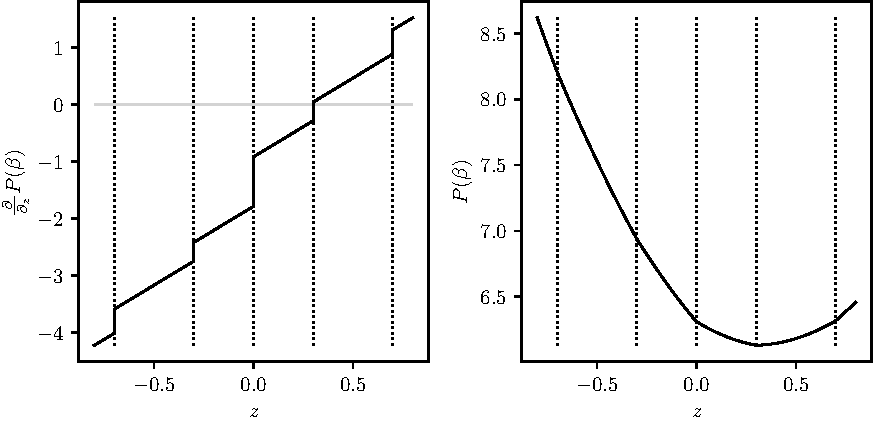
\includegraphics[]{clusterupdate-grad-obj}
  \caption{%
    Objective and gradient under the constraint that we have a fixed
    cluster.
    The optimum is found at \(\alpha = 0.3\).
  }%
  \label{fig:cluster-grad-obj}
\end{figure}

We are now ready to introduce a solution to~\eqref{eq:cluster-problem}, using
the SLOPE thresholding operator~\cref{thm:slope-thresholding}.

\begin{theorem}
  \label{thm:slope-thresholding}
  Let
  \begin{multline*}
    T_k(\gamma, \omega; c, \lambda) = \\
    \begin{cases}
      0                                                                         &
      \splitfrac{
        \text{if } \big(-\sum_{j = p - p_k + 1}^p \lambda_j < \gamma \leq \sum_{j = p - p_k + 1}^p \lambda_j
        \text{ and } c_m \neq 0\big)
      }{%
        \text{ or } \big(  -\sum_{j = p - p_k - p_m + 1}^{p - p_m} \lambda_j < \gamma \leq \sum_{j = p - p_k + 1}^{p_m} \lambda_j \text{ and } c_m = 0\big),
      }                                                                                                                                                                                                                    \\
      c_i                                                                       & \text{if } \exists\, i \neq k: \sum_{j = b_i - p_k + 1}^{b_i} \lambda_j \leq \gamma - \omega c_i \leq \sum_{j = a_i}^{p_k} \lambda_j,    \\
      -c_i                                                                      & \text{if } \exists\, i \neq k : \sum_{j = b_i - p_k + 1}^{b_i} \lambda_j \leq - \gamma - \omega c_i \leq \sum_{j = a_i}^{p_k} \lambda_j, \\
      \frac{1}{\omega}\left(\gamma - \sum_{j \in C(z)} \lambda_{(j)^-_z}\right) & \text{otherwise.}                                                                                                                        \\
    \end{cases}
  \end{multline*}
  A minimizer for \eqref{eq:cluster-problem} is given by \(T_k(\tilde{r}^T\tilde{x}, \tilde{x}^T\tilde{x}; c, \lambda)\).
\end{theorem}
\begin{proof}
  Let \(\gamma = \tilde{r}^T\tilde{x}\) and \(\omega = \tilde{x}^T\tilde{x}\).
  For a minimizer to~\eqref{eq:cluster-problem}, the optimality condition is
  \[
    0 \in \tilde{x}^T\tilde{x} z - \tilde{r}^T \tilde{x} + \partial J_k(z).
  \]
  \(z = c_i \neq 0\) is a minimizer of~\eqref{eq:cluster-problem} if and only if
  \[
    0 \in \omega c_i - \gamma +
    \left[\sum_{j = b_i - p_k + 1}^{b_i} \lambda_j, \sum_{j=a_i}^{p_k}\lambda_j \right],
  \]
  which is equivalent to
  \[
    \smashoperator[r]{\sum_{j = b_i - p_k + 1}^{b_i}} \lambda_j \leq \gamma - \omega c_i \leq \sum_{j = a_i}^{p_k} \lambda_j.
  \]
  \(z = -c_i \neq 0\) is a minimizer of~\eqref{eq:cluster-problem} if and only if
  \[
    0 \in -\omega c_i - \gamma +
    \left[-\sum_{j=a_i}^{p_k}\lambda_j, -\smashoperator{\sum_{j = b_i - p_k + 1}^{b_i}} \lambda_j\,\right],
  \]
  which is equivalent to
  \[
    \smashoperator[r]{\sum_{j = b_i - p_k + 1}^{b_i}} \lambda_j \leq -\gamma - \omega c_i \leq \sum_{j = a_i}^{p_k} \lambda_j.
  \]
  If \(c_m \neq 0\), then \(z = 0\) is a minimizer if
  \[
    0 \in -\gamma +
    \left[-\sum_{j = p - p_k + 1}^{p} \lambda_j, \sum_{j=p - p_k + 1}^{p}\lambda_j \right],
  \]
  which is equivalent to
  \[
    -\sum_{j = p - p_k + 1}^{p} \lambda_j \leq \gamma \leq \sum_{j = p - p_k + 1}^{p} \lambda_j.
  \]
  Finally, if \(c_m = 0\), then \(z = 0\) is a minimizer if
  \[
    0 \in -\gamma +
    \left[
      -\sum_{j = p - p_k - p_m + 1}^{p - p_m} \lambda_j,
      \sum_{j=p - p_k - p_m + 1}^{p - p_m}\lambda_j
      \right],
  \]
  which is equivalent to
  \[
    -\sum_{j = p - p_k + 1}^{p} \lambda_j \leq \gamma \leq \sum_{j = p - p_k + 1}^{p} \lambda_j.
  \]


\end{proof}

\begin{equation}
  \label{eq:slope-thresholding}
  T(a, \lambda,k,\tilde \beta, \mathcal{C}) =
  \begin{cases}
    0                                                                 & \text{if } |a| \leq \sum_{i=1}^{|\mathcal{C}_k|}\lambda^{C_0}_i                                                                                                                               \\
    \sign(a)|\tilde \beta_i|                                          & \text{if } \sum_{j= |\mathcal{C}_i| - |\mathcal{C}_k| + 1}^{|\mathcal{C}_i|} \lambda^{\mathcal{C}_i}_j \leq |a| - |\tilde \beta_i| \leq \sum_{j=1}^{|\mathcal{C}_k|}\lambda^{\mathcal{C}_i}_j \\
    \sign(a)\big(|a| - \sum_{j \in \mathcal{C}_k}\lambda_{(j)^-}\big) & \text{otherwise.
    }
  \end{cases}
\end{equation}
To emphasize the connection between \(T\) and the soft-thresholding operator
for the lasso, we call this operator the SLOPE-thresholding operator.
In \cref{fig:slope-thresholding}, we visualize the operator.

\begin{figure}[htbp]
  \centering
  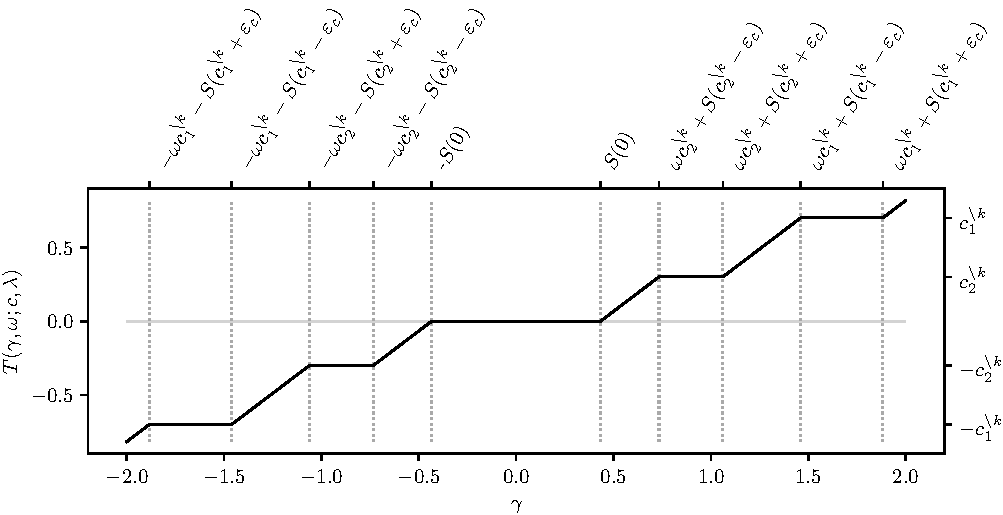
\includegraphics[]{slope-thresholding.pdf}
  \caption{The result of the SLOPE thresholding update.}
  \label{fig:slope-thresholding}
\end{figure}

\subsubsection{Naive Updates}

As in \textcite{friedman2010}, we can improve the efficiency of updates by observing that
\begin{equation*}
  \begin{aligned}
    \tilde r_k & = y - \tilde y_k                                                                       \\
               & = y - X_{\bar{\mathcal{C}}_k}\beta_{\bar{\mathcal{C}}_k} - \tilde x c_k + \tilde x c_k \\
               & = r + \tilde x c_k
  \end{aligned}
\end{equation*}
and therefore that
\begin{equation}
  \label{eq:naive-update}
  \tilde x_k^T (y - \tilde y_k) = \tilde x_k^T r + \tilde x_k^T \tilde x_k c_k.
\end{equation}

\subsubsection{Caching Reductions}

Observe that \(\tilde x_k\) only changes between subsequent coordinate updates provided that the members of the cluster \(k\) change, for instance if two clusters are merged, a predictor leaves a cluster, or the signs flip (through an update of \(\alpha_k\)).
As a result, it is possible to obtain computational gains by caching \(\tilde x_k\) and \(\tilde x_k^T \tilde x_k\) for each cluster (except the zero cluster, which we do not consider in our coordinate descent step).
When there is no change in the clusters, there is no need to recompute these quantities.
And even when there are changes, we can still reduce the costs involved since \(\tilde x_k\) can be updated in place.
If a large cluster is joined by few new predictors, then the cost of updating may be much lower than recomputing the quantities for the entire cluster.
Also note that, for single-member clusters we only need to store \(\tilde x_k^T \tilde x_k\) since \(\tilde x_k\) is just a column in \(X\) times the corresponding sign.

Letting \(\tilde x_k^\text{old}\) correspond to the value of \(\tilde x_k\) before the update, we note that \(\tilde x_k \gets \tilde x_k^\text{old} + x_j \sign(\beta_j)\) for each \(j \in \mathcal{C}_k^\text{new} \setminus \mathcal{C}_k^\text{old}\) and \(\tilde x_k \gets \tilde x_k^\text{old} - x_j \sign(\beta_j)\) for each \(j \in \mathcal{C}_k^\text{old} \setminus \mathcal{C}_k^\text{new}\).
If only the signs flip, we simply have to also flip the signs in \(\tilde x_k\).

\subsubsection{Covariance Updates}

Notice that we can rewrite the first term in \eqref{eq:naive-update} as
\begin{equation}
  \begin{aligned}
    \tilde x_k^T r & = \tilde x_k^T y - \sum_{j : \beta_j \neq 0} \tilde x_k^T x_j \beta_j                                                                    \\
                   & = \tilde x_k^T y - \sum_{j : c_j \neq 0} \tilde x_k^T \tilde x_j c_j                                                                     \\
                   & = s_{\mathcal{C}_k}^T X_{\mathcal{C}_k}^T y - \sum_{j : \beta_j \neq 0} s_{\mathcal{C}_k}^T X_{\mathcal{C}_k}^T x_j \beta_j              \\
                   & = s_{\mathcal{C}_k}^T \left(X^T y\right)_{\mathcal{C}_k} - \sum_{j : \beta_j \neq 0} s_{\mathcal{C}_k}^T X_{\mathcal{C}_k}^T x_j \beta_j \\
                   & = \sum_{j \in \mathcal{C}_k}\left( s_j x_j^Ty - \sum_{t : \beta_t \neq 0} s_j x_j^T x_t \beta_t \right)
  \end{aligned}
\end{equation}
As in \textcite{friedman2010}, this formulation can be used to achieve so-called \emph{covariance updates}.
We compute \(X^T y\) once at the start.
Then, each time a new predictor becomes non-zero, we compute its inner product with all other predictors, caching these products.

\subsection{Hybrid proximal coordinate descent strategy}

We propose an iterative solver that alternates between proximal gradient step and proximal coordinate descent.
Since the regularization term for SLOPE is not separable, applying PCD does not guarantee convergence (show example where CD gets stuck).
However, \cite{dupuis2021} showed that once the clusters are known, the subdifferential of $J$ can be written as the cartesian product of the subdifferential of $J$ restricted to the clusters.
Hence, if one knew the clusters, PCD updates could be applied on each cluster.

The notion of clusters for SLOPE extends the notion of sparsity coming from the LASSO.
Identification of the sparsity pattern throughout the iterative algorithm have largely been studied.
Talk about Partly Smooth functions, related Manifold and that support transpose to cluster for SLOPE regularization. DO the maths.

Then identification of this underlying structure occurs when applying PGD.
Hence the idea to alternate, PGD and PCD step to take advantage of the speed of PCD and ensure convergence via the identification of the right structure with PGD steps.

\begin{algorithm}[tb]
  \SetKwInOut{Init}{init}
  \SetKwInOut{Input}{input}
  \caption{%
    Hybrid coordinate descent and proximal gradient descent algorithm
    for SLOPE\label{alg:hybrid}}
  \Input{
    \(X \in \mathbb{R}^{n\times p}, y\in \mathbb{R}^n, \beta\in \mathbb{R}^p, \lambda \in \{\mathbb{R}^p : \lambda_1 \geq \lambda_2 \geq \cdots > 0\}\), \(m \in \mathbb{N}\)}

  \Init{\(t \gets 0\), \(\beta \gets 0\), \(L \gets \lVert X \rVert_2^2\)}

  \Repeat{convergence}{
  \(t \gets t + 1\)

  \If{\(t \bmod m = 0\)}{

  \(\beta \leftarrow \operatorname{prox}_{J / L}(\beta - \frac{1}{L}\nabla f(\beta))\) \label{alg:hybrid-istastep}

  % \(C_1, \hdots, C_m \leftarrow \mathtt{get\_clusters}(\beta)\)
  }
  \Else{
    \(k \gets 0\)

    \While{\(k \leq \lvert \mathcal{C} \rvert\)}{
      \(k \gets k + 1\)

      \(s \leftarrow \mathrm{sign}(\beta_{\mathcal{C}_k})\)

      \If{\(s \neq 0\)}{
        % \(L_k \gets (X_{:, \mathcal{C}_k}s)^\top  X_{:, \mathcal{C}_k}s\)


        % \(\tilde{\beta} \gets T(|\beta_{\mathcal{C}_k}| - \frac{1}{L_k} \nabla_{\mathcal{C}_k}f(\beta)^\top s, \frac{\lambda}{L_k})\)

        % \(\beta_{\mathcal{C}_k} \leftarrow \tilde{\beta} s\)
        \(\tilde x_k \gets X_{\mathcal{C}_k}s\)

        \(\tilde y_k \gets X_{\widebar{\mathcal{C}}_k}\beta_{\widebar{\mathcal{C}}_k}\)

        \(\tilde r_k \gets y - \tilde y_k\)

        \(
        \beta_{\mathcal{C}_k} \gets
        s T \left(
        \frac{\tilde r^T_k \tilde x_k, }{ \tilde x_k^T \tilde x_k},
        \frac{\lambda}{ \tilde x_k^T \tilde x_k},
        k,
        \tilde \beta,
        \mathcal{C}
        \right)
        \)
        \Comment{\(\mathcal{C}\) is updated at this step.}


      }

    }
  }

  }
  \Return{\(\beta\)}
\end{algorithm}

In \cref{fig:illustration-solver}, we show how \cref{alg:hybrid} works in practice on
a two-dimensional SLOPE problem.

\begin{figure}[htbp]
  \centering
  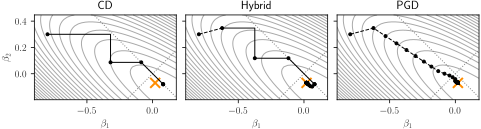
\includegraphics{illustration_solvers}
  \caption{Illustration of the proposed solver. These figures show ten epochs of
    the coordinate descent (CD) solver that we use as part of the hybrid method,
    our hybrid method, or proximal gradient descent (PGD). The orange cross marks
    the optimum. The dotted lines indicate where the coefficients are equal
    in absolute value. Each dot marks a complete epoch, which may correspond to only
    a single coefficient update for the CD and hybrid solvers if the coefficients
    flip order.}
  \label{fig:illustration-solver}
\end{figure}

\begin{theorem}
  Iterates of \cref{alg:hybrid} converge towards \(\beta^*\).
\end{theorem}
\begin{proof}
  First note that convergence properties of proximal gradient descent on convex
  problems such as SLOPE are well-established
  \parencite{beck2009,daubechies2004}, which certifies that updates via
  \cref{alg:hybrid-istastep} make progress towards \(\beta^*\).

  Next note that the objectives of \eqref{pb:slope} and
  \eqref{eq:subproblem} are equal and that \eqref{eq:subproblem} can be seen
  viewed as a version of \eqref{pb:slope} with added linear constraints
  that is also convex. And, finally, because the coordinate updates of
  \cref{alg:hybrid} minimize the sub-problem, we in the worst case make no
  progress and therefore have guaranteed converge rate no less than \(1/m\)
  of that of proximal gradient descent.
\end{proof}

